\documentclass{article}\usepackage{graphicx, color}
%% maxwidth is the original width if it is less than linewidth
%% otherwise use linewidth (to make sure the graphics do not exceed the margin)
\makeatletter
\def\maxwidth{ %
  \ifdim\Gin@nat@width>\linewidth
    \linewidth
  \else
    \Gin@nat@width
  \fi
}
\makeatother

\IfFileExists{upquote.sty}{\usepackage{upquote}}{}
\definecolor{fgcolor}{rgb}{0.2, 0.2, 0.2}
\newcommand{\hlnumber}[1]{\textcolor[rgb]{0,0,0}{#1}}%
\newcommand{\hlfunctioncall}[1]{\textcolor[rgb]{0.501960784313725,0,0.329411764705882}{\textbf{#1}}}%
\newcommand{\hlstring}[1]{\textcolor[rgb]{0.6,0.6,1}{#1}}%
\newcommand{\hlkeyword}[1]{\textcolor[rgb]{0,0,0}{\textbf{#1}}}%
\newcommand{\hlargument}[1]{\textcolor[rgb]{0.690196078431373,0.250980392156863,0.0196078431372549}{#1}}%
\newcommand{\hlcomment}[1]{\textcolor[rgb]{0.180392156862745,0.6,0.341176470588235}{#1}}%
\newcommand{\hlroxygencomment}[1]{\textcolor[rgb]{0.43921568627451,0.47843137254902,0.701960784313725}{#1}}%
\newcommand{\hlformalargs}[1]{\textcolor[rgb]{0.690196078431373,0.250980392156863,0.0196078431372549}{#1}}%
\newcommand{\hleqformalargs}[1]{\textcolor[rgb]{0.690196078431373,0.250980392156863,0.0196078431372549}{#1}}%
\newcommand{\hlassignement}[1]{\textcolor[rgb]{0,0,0}{\textbf{#1}}}%
\newcommand{\hlpackage}[1]{\textcolor[rgb]{0.588235294117647,0.709803921568627,0.145098039215686}{#1}}%
\newcommand{\hlslot}[1]{\textit{#1}}%
\newcommand{\hlsymbol}[1]{\textcolor[rgb]{0,0,0}{#1}}%
\newcommand{\hlprompt}[1]{\textcolor[rgb]{0.2,0.2,0.2}{#1}}%

\usepackage{framed}
\makeatletter
\newenvironment{kframe}{%
 \def\at@end@of@kframe{}%
 \ifinner\ifhmode%
  \def\at@end@of@kframe{\end{minipage}}%
  \begin{minipage}{\columnwidth}%
 \fi\fi%
 \def\FrameCommand##1{\hskip\@totalleftmargin \hskip-\fboxsep
 \colorbox{shadecolor}{##1}\hskip-\fboxsep
     % There is no \\@totalrightmargin, so:
     \hskip-\linewidth \hskip-\@totalleftmargin \hskip\columnwidth}%
 \MakeFramed {\advance\hsize-\width
   \@totalleftmargin\z@ \linewidth\hsize
   \@setminipage}}%
 {\par\unskip\endMakeFramed%
 \at@end@of@kframe}
\makeatother

\definecolor{shadecolor}{rgb}{.97, .97, .97}
\definecolor{messagecolor}{rgb}{0, 0, 0}
\definecolor{warningcolor}{rgb}{1, 0, 1}
\definecolor{errorcolor}{rgb}{1, 0, 0}
\newenvironment{knitrout}{}{} % an empty environment to be redefined in TeX

\usepackage{alltt}

\begin{document}


\section*{Dissolved CO2 measurement and other physical parameters}



\begin{knitrout}
\definecolor{shadecolor}{rgb}{0.969, 0.969, 0.969}\color{fgcolor}\begin{kframe}
\begin{alltt}
\hlcomment{# Housekeeping}
sweave.dir <- \hlfunctioncall{getwd}()
\hlfunctioncall{library}(ggplot2)
\hlfunctioncall{library}(plyr)
\hlfunctioncall{library}(reshape)
\end{alltt}
\begin{flushleft}\ttfamily\noindent\itshape\textcolor{messagecolor}{\#\# Attaching package: 'reshape'}\end{flushleft}\begin{flushleft}\ttfamily\noindent\itshape\textcolor{messagecolor}{\#\# The following object(s) are masked from 'package:plyr': \\ 
\#\#  \\ 
\#\# rename, round\_any}\end{flushleft}\begin{alltt}
\hlfunctioncall{library}(devtools)
\end{alltt}
\begin{flushleft}\ttfamily\noindent\textcolor{warningcolor}{\#\# Warning: package 'devtools' was built under R version 2.15.1}\end{flushleft}\begin{alltt}
\hlfunctioncall{library}(gridExtra)
\end{alltt}
\begin{flushleft}\ttfamily\noindent\textcolor{warningcolor}{\#\# Warning: package 'gridExtra' was built under R version 2.15.1}\end{flushleft}\begin{flushleft}\ttfamily\noindent\itshape\textcolor{messagecolor}{\#\# Loading required package: grid}\end{flushleft}\begin{alltt}
\hlfunctioncall{setwd}(\hlstring{"~/Dropbox/co2_selection"})
\hlfunctioncall{source_url}(\hlstring{"https://raw.github.com/edielivon/Useful-R-functions/master/Growth%20curves/00_source_all.R"})
\end{alltt}
\begin{flushleft}\ttfamily\noindent\bfseries\textcolor{errorcolor}{\#\# Error: http client error (404)}\end{flushleft}\begin{alltt}
\hlfunctioncall{source_url}(\hlstring{"https://raw.github.com/gist/2594954/6f664f27315cf4d2e202329975935afaf60b466d/ggplot2%20theme_minimal"})


CO2 <- CO2[CO2$period == 1 | CO2$period == 6]

\hlcomment{# Load data}
\hlfunctioncall{load}(file = \hlstring{"./Outputs/CO2media.RData"})

\hlfunctioncall{setwd}(sweave.dir)
\end{alltt}
\end{kframe}
\end{knitrout}


\begin{knitrout}
\definecolor{shadecolor}{rgb}{0.969, 0.969, 0.969}\color{fgcolor}\begin{kframe}
\begin{flushleft}\ttfamily\noindent\itshape\textcolor{messagecolor}{\#\# geom\_smooth: method="auto" and size of largest group is <1000, so using \\ 
\#\# loess. Use 'method = x' to change the smoothing method.}\end{flushleft}\begin{flushleft}\ttfamily\noindent\itshape\textcolor{messagecolor}{\#\# geom\_smooth: method="auto" and size of largest group is <1000, so using \\ 
\#\# loess. Use 'method = x' to change the smoothing method.}\end{flushleft}\begin{flushleft}\ttfamily\noindent\itshape\textcolor{messagecolor}{\#\# geom\_smooth: method="auto" and size of largest group is <1000, so using \\ 
\#\# loess. Use 'method = x' to change the smoothing method.}\end{flushleft}\begin{flushleft}\ttfamily\noindent\itshape\textcolor{messagecolor}{\#\# geom\_smooth: method="auto" and size of largest group is <1000, so using \\ 
\#\# loess. Use 'method = x' to change the smoothing method.}\end{flushleft}\begin{flushleft}\ttfamily\noindent\itshape\textcolor{messagecolor}{\#\# geom\_smooth: method="auto" and size of largest group is <1000, so using \\ 
\#\# loess. Use 'method = x' to change the smoothing method.}\end{flushleft}\begin{flushleft}\ttfamily\noindent\itshape\textcolor{messagecolor}{\#\# geom\_smooth: method="auto" and size of largest group is <1000, so using \\ 
\#\# loess. Use 'method = x' to change the smoothing method.}\end{flushleft}\end{kframe}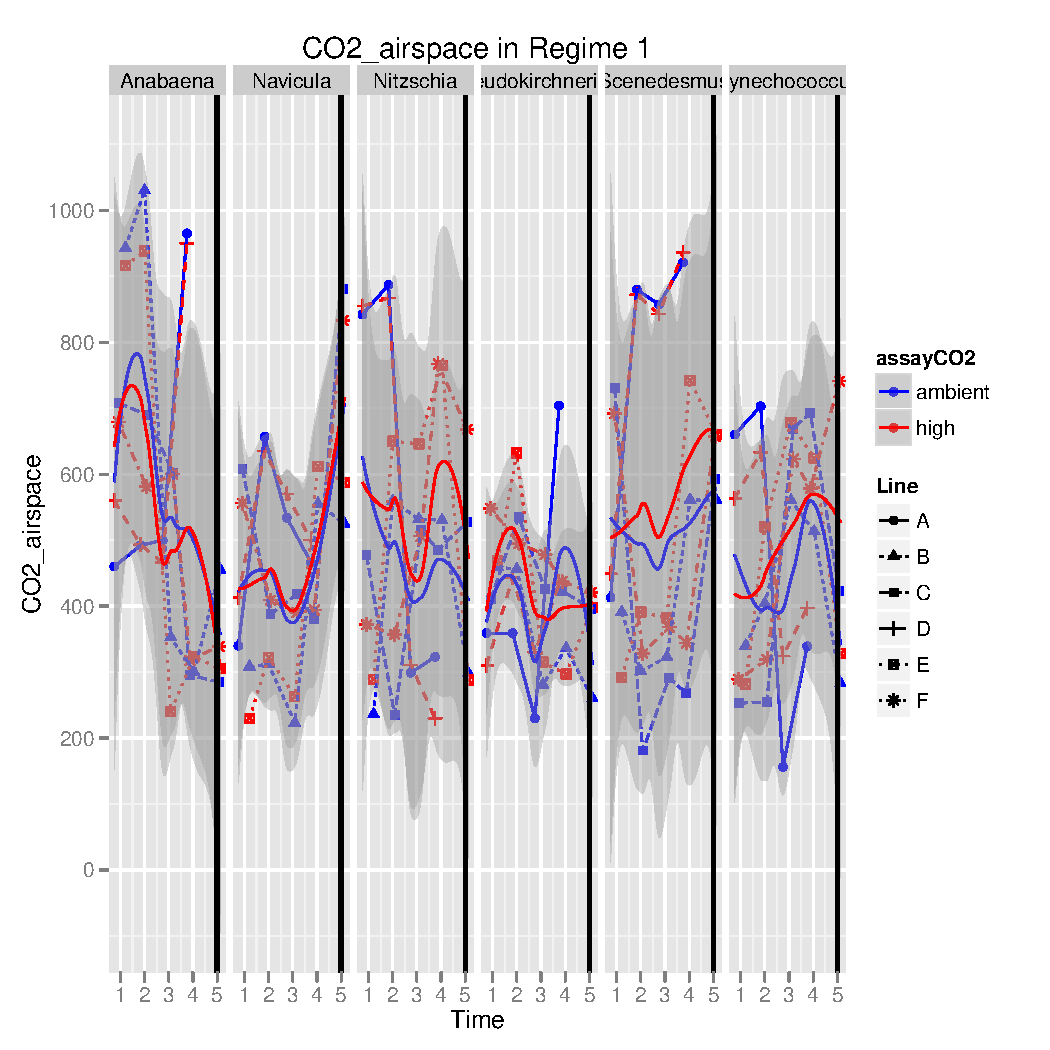
\includegraphics[width=\maxwidth]{figure/physical_parameters_figure1} \begin{kframe}\begin{flushleft}\ttfamily\noindent\itshape\textcolor{messagecolor}{\#\# geom\_smooth: method="auto" and size of largest group is <1000, so using \\ 
\#\# loess. Use 'method = x' to change the smoothing method.}\end{flushleft}\begin{flushleft}\ttfamily\noindent\itshape\textcolor{messagecolor}{\#\# geom\_smooth: method="auto" and size of largest group is <1000, so using \\ 
\#\# loess. Use 'method = x' to change the smoothing method.}\end{flushleft}\begin{flushleft}\ttfamily\noindent\itshape\textcolor{messagecolor}{\#\# geom\_smooth: method="auto" and size of largest group is <1000, so using \\ 
\#\# loess. Use 'method = x' to change the smoothing method.}\end{flushleft}\begin{flushleft}\ttfamily\noindent\itshape\textcolor{messagecolor}{\#\# geom\_smooth: method="auto" and size of largest group is <1000, so using \\ 
\#\# loess. Use 'method = x' to change the smoothing method.}\end{flushleft}\begin{flushleft}\ttfamily\noindent\itshape\textcolor{messagecolor}{\#\# geom\_smooth: method="auto" and size of largest group is <1000, so using \\ 
\#\# loess. Use 'method = x' to change the smoothing method.}\end{flushleft}\begin{flushleft}\ttfamily\noindent\itshape\textcolor{messagecolor}{\#\# geom\_smooth: method="auto" and size of largest group is <1000, so using \\ 
\#\# loess. Use 'method = x' to change the smoothing method.}\end{flushleft}\end{kframe}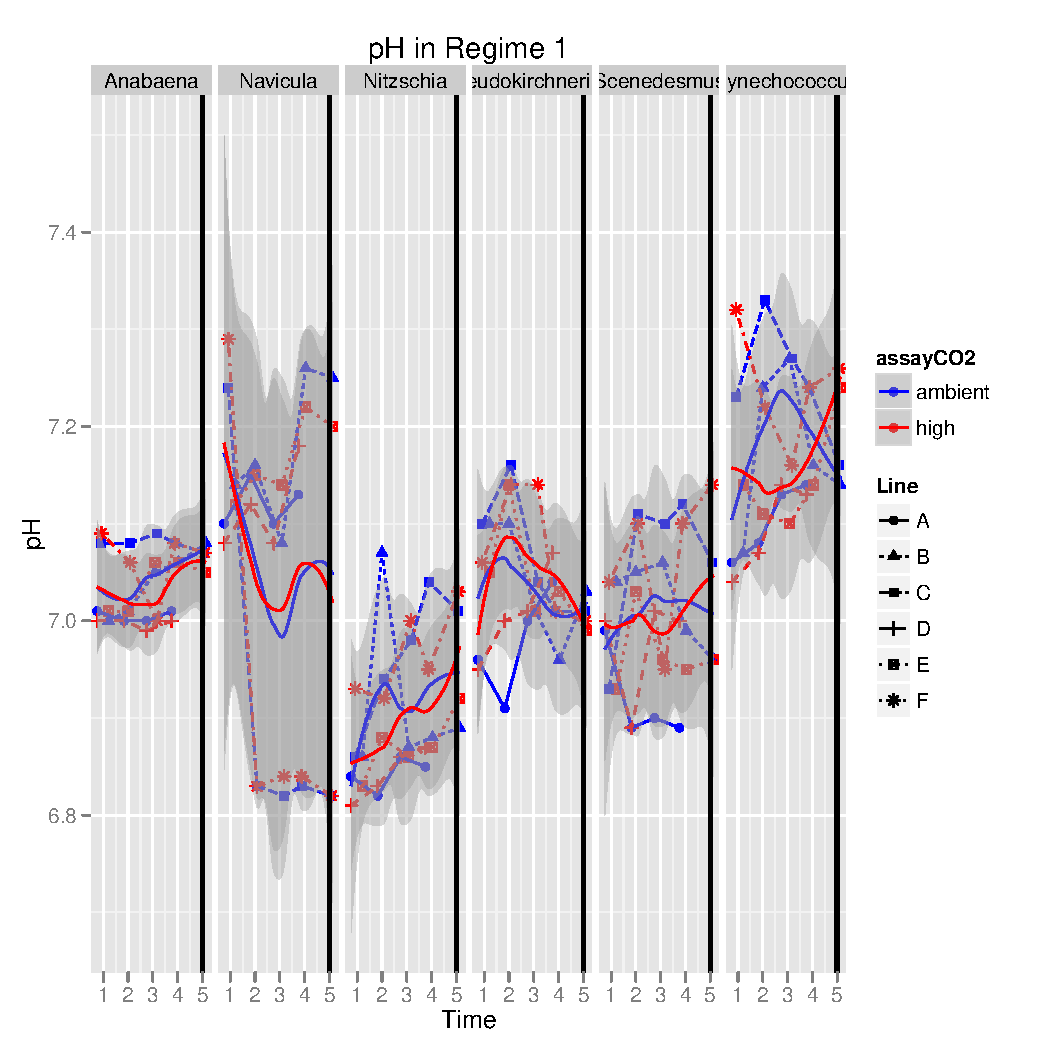
\includegraphics[width=\maxwidth]{figure/physical_parameters_figure2} \begin{kframe}\begin{flushleft}\ttfamily\noindent\itshape\textcolor{messagecolor}{\#\# geom\_smooth: method="auto" and size of largest group is <1000, so using \\ 
\#\# loess. Use 'method = x' to change the smoothing method.}\end{flushleft}\begin{flushleft}\ttfamily\noindent\itshape\textcolor{messagecolor}{\#\# geom\_smooth: method="auto" and size of largest group is <1000, so using \\ 
\#\# loess. Use 'method = x' to change the smoothing method.}\end{flushleft}\begin{flushleft}\ttfamily\noindent\itshape\textcolor{messagecolor}{\#\# geom\_smooth: method="auto" and size of largest group is <1000, so using \\ 
\#\# loess. Use 'method = x' to change the smoothing method.}\end{flushleft}\begin{flushleft}\ttfamily\noindent\itshape\textcolor{messagecolor}{\#\# geom\_smooth: method="auto" and size of largest group is <1000, so using \\ 
\#\# loess. Use 'method = x' to change the smoothing method.}\end{flushleft}\begin{flushleft}\ttfamily\noindent\itshape\textcolor{messagecolor}{\#\# geom\_smooth: method="auto" and size of largest group is <1000, so using \\ 
\#\# loess. Use 'method = x' to change the smoothing method.}\end{flushleft}\begin{flushleft}\ttfamily\noindent\itshape\textcolor{messagecolor}{\#\# geom\_smooth: method="auto" and size of largest group is <1000, so using \\ 
\#\# loess. Use 'method = x' to change the smoothing method.}\end{flushleft}\end{kframe}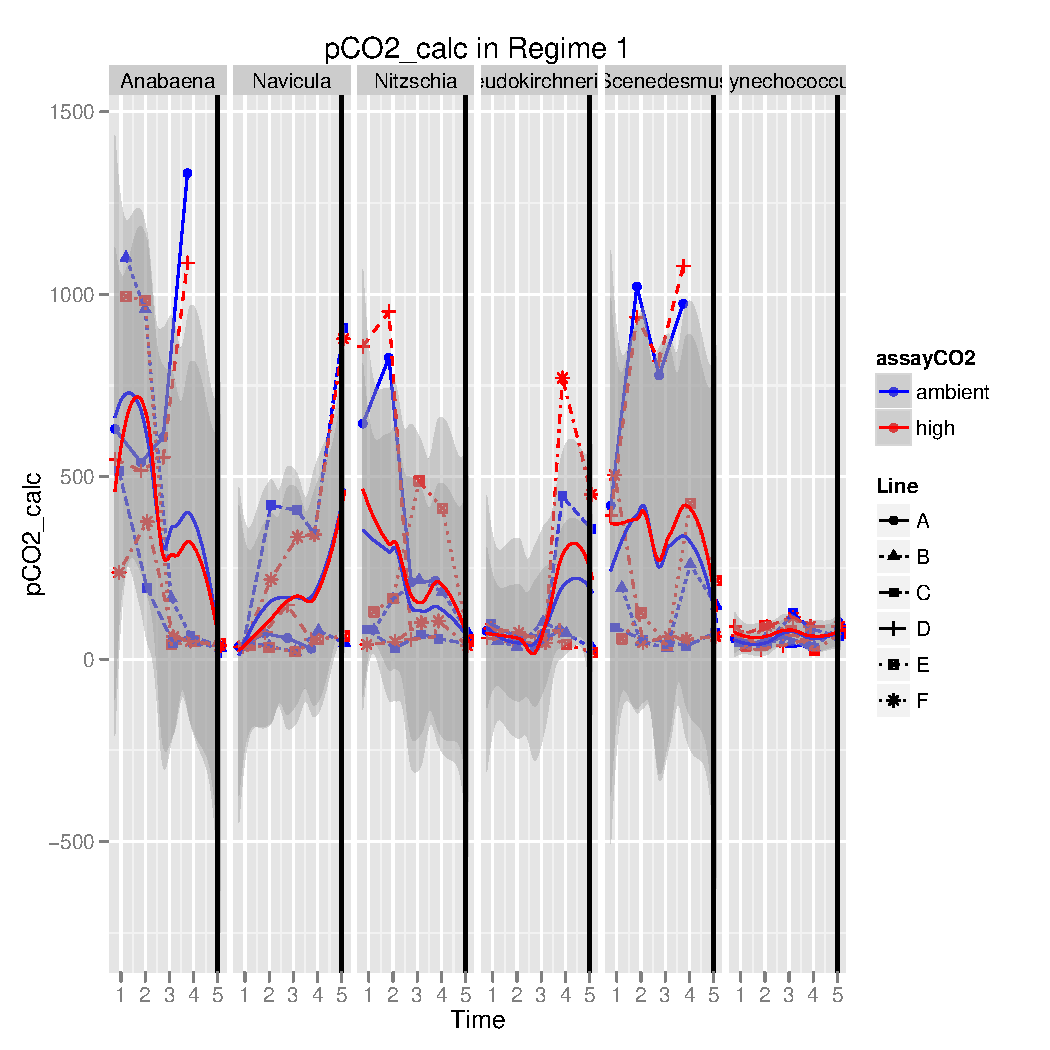
\includegraphics[width=\maxwidth]{figure/physical_parameters_figure3} 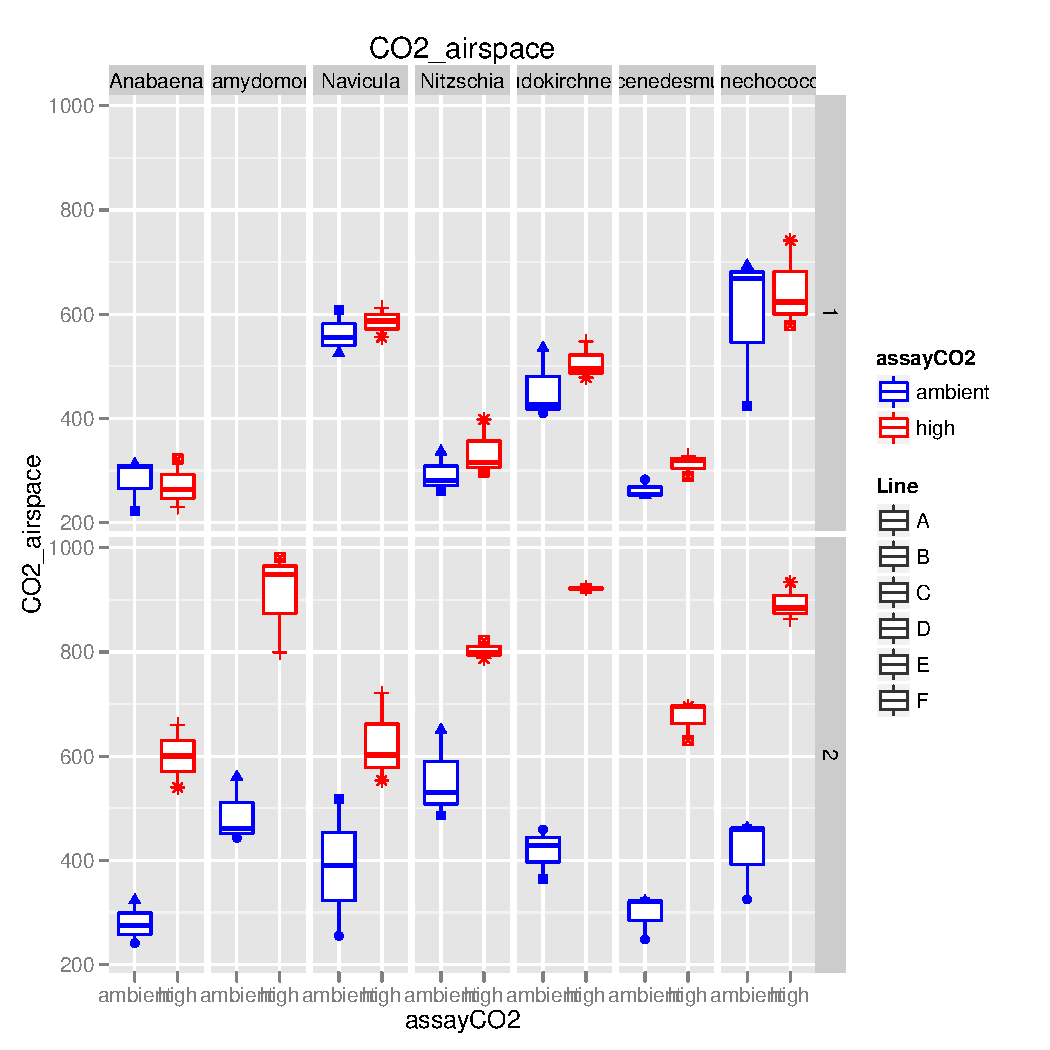
\includegraphics[width=\maxwidth]{figure/physical_parameters_figure4} 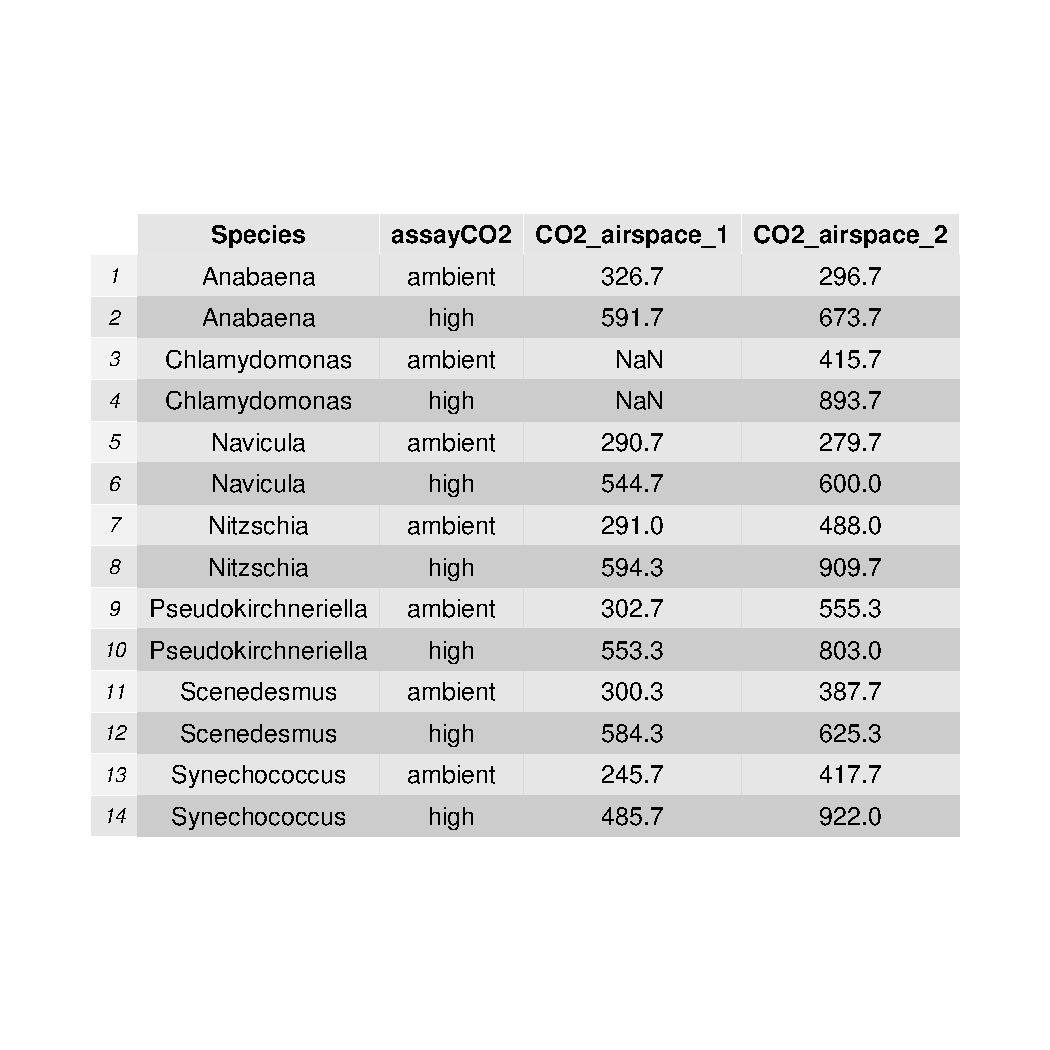
\includegraphics[width=\maxwidth]{figure/physical_parameters_figure5} 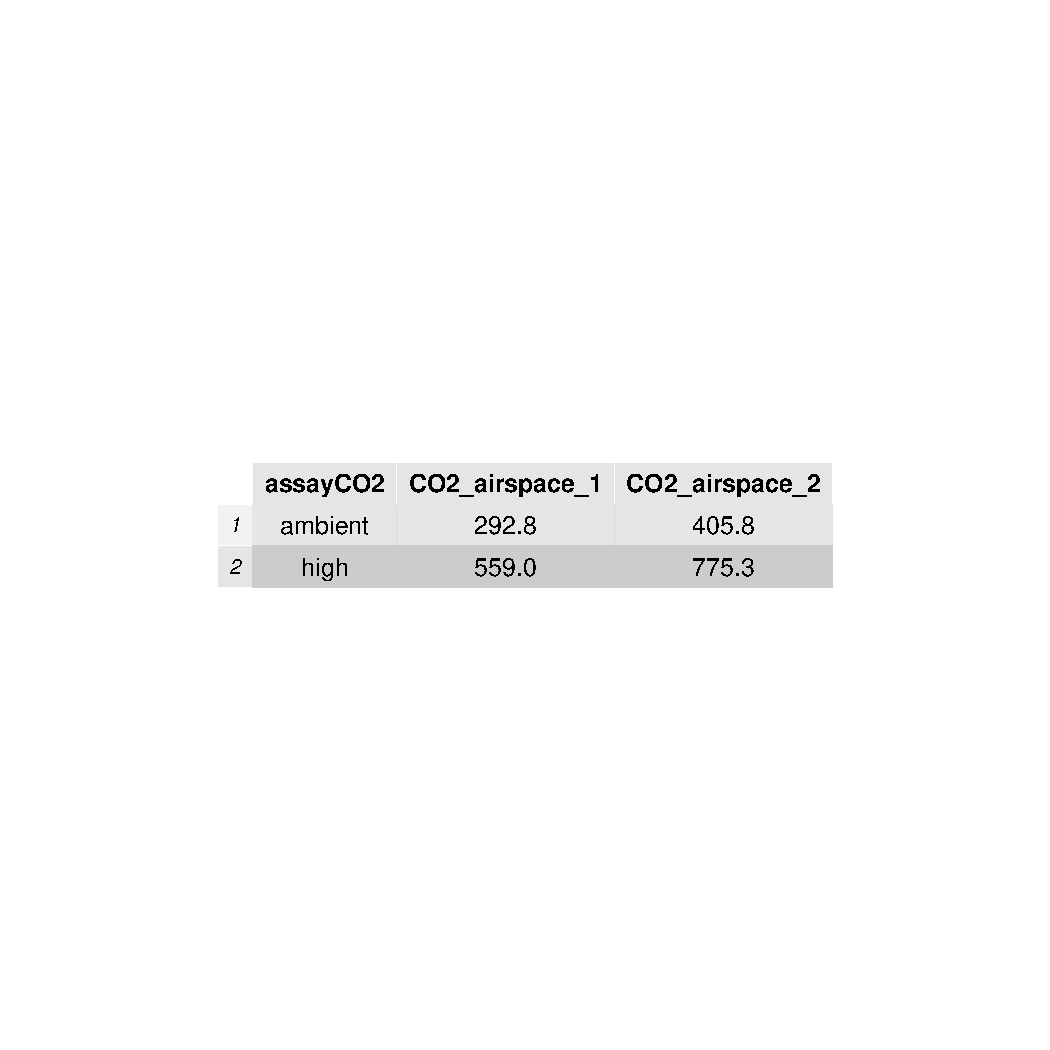
\includegraphics[width=\maxwidth]{figure/physical_parameters_figure6} 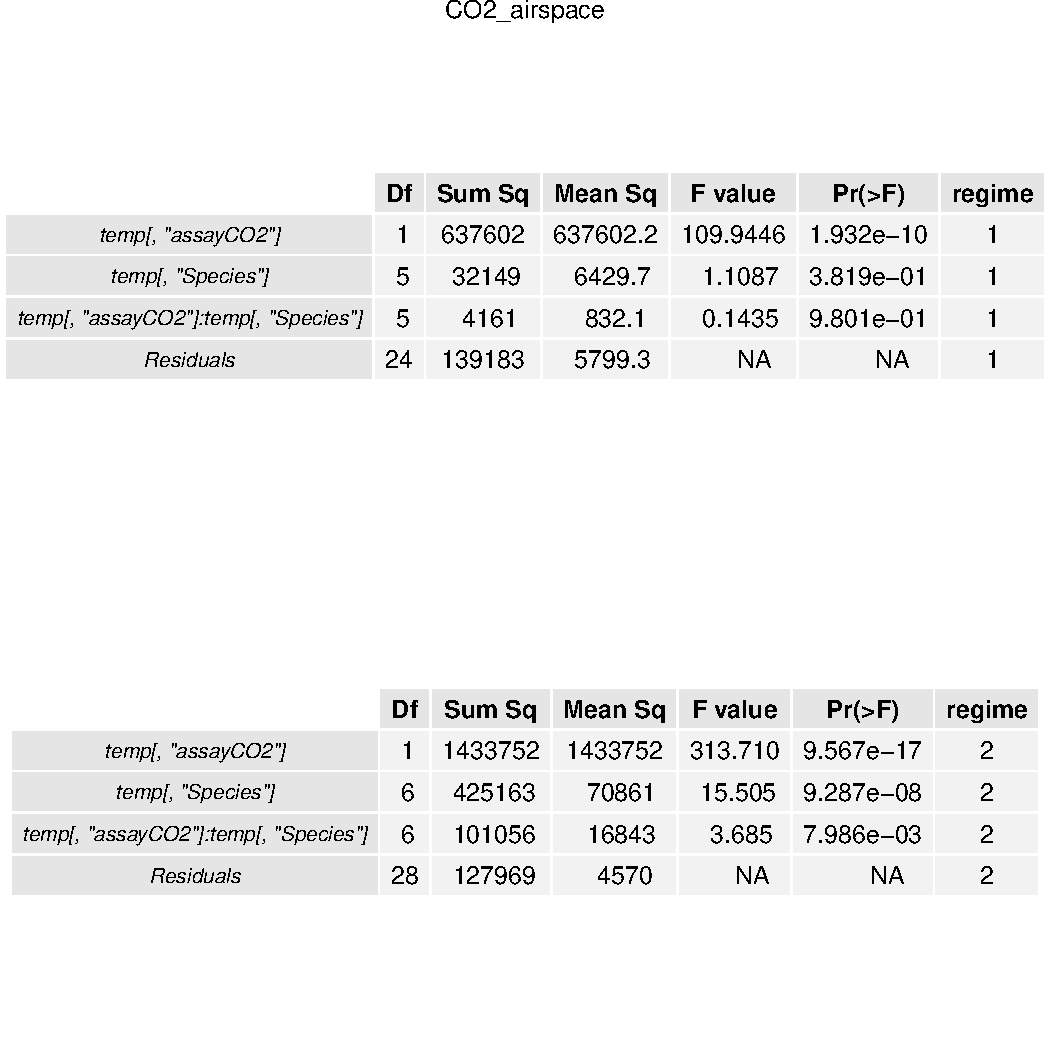
\includegraphics[width=\maxwidth]{figure/physical_parameters_figure7} 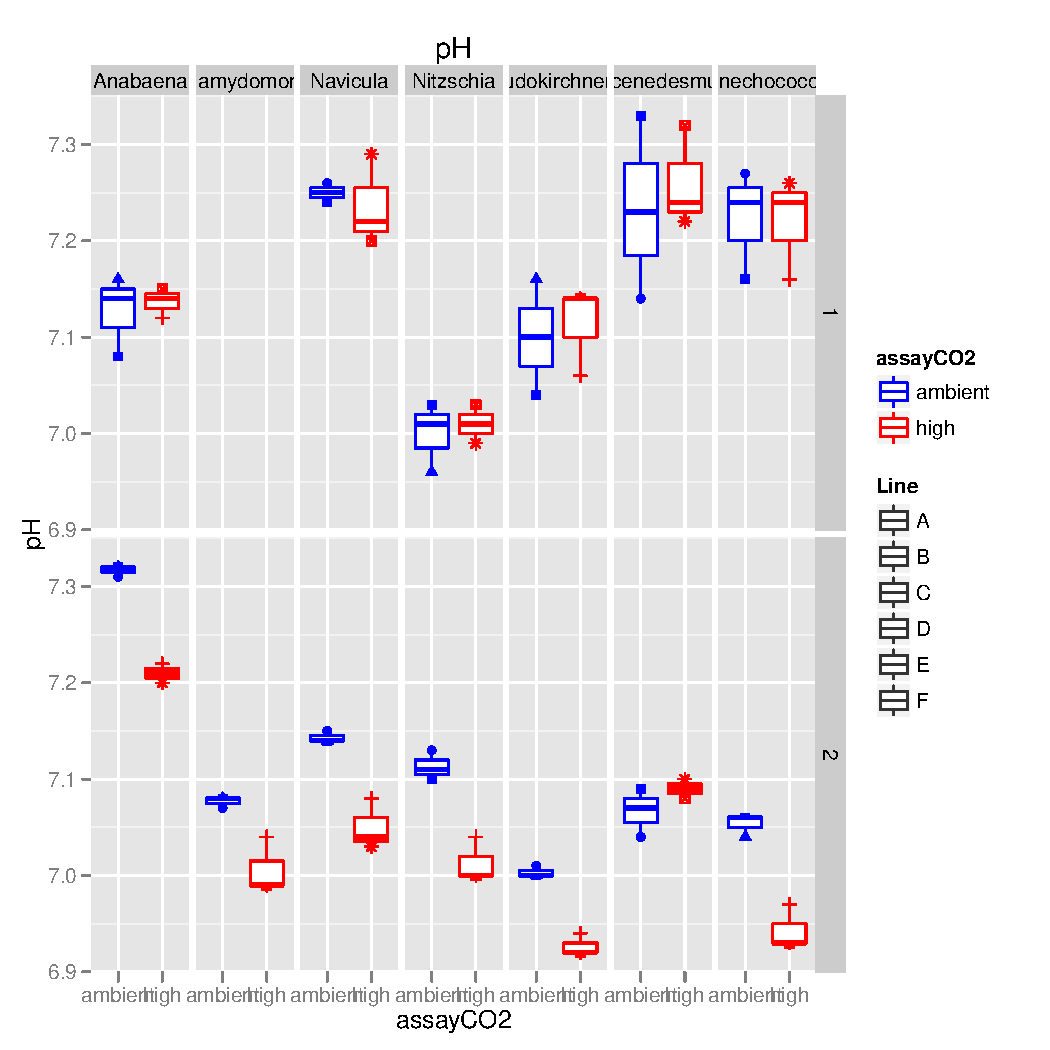
\includegraphics[width=\maxwidth]{figure/physical_parameters_figure8} 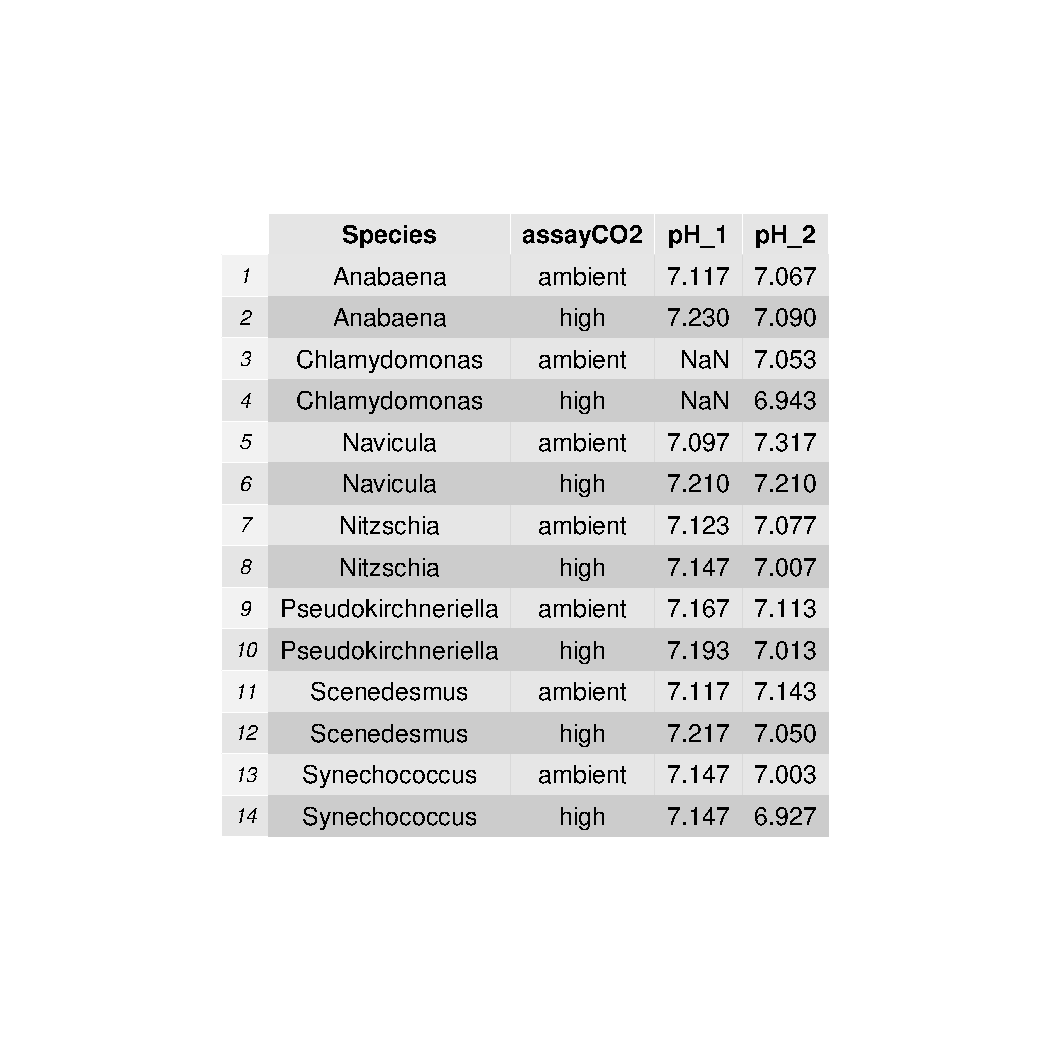
\includegraphics[width=\maxwidth]{figure/physical_parameters_figure9} 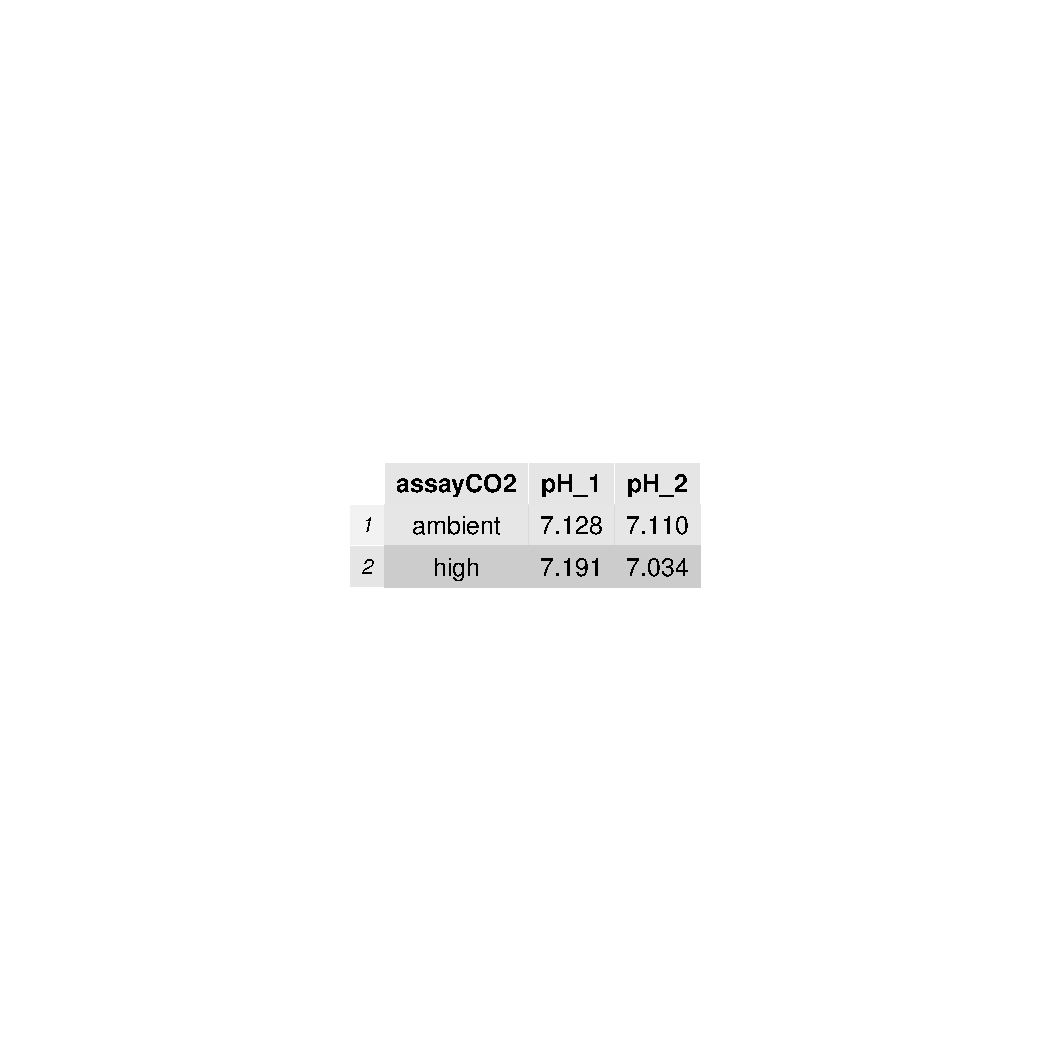
\includegraphics[width=\maxwidth]{figure/physical_parameters_figure10} 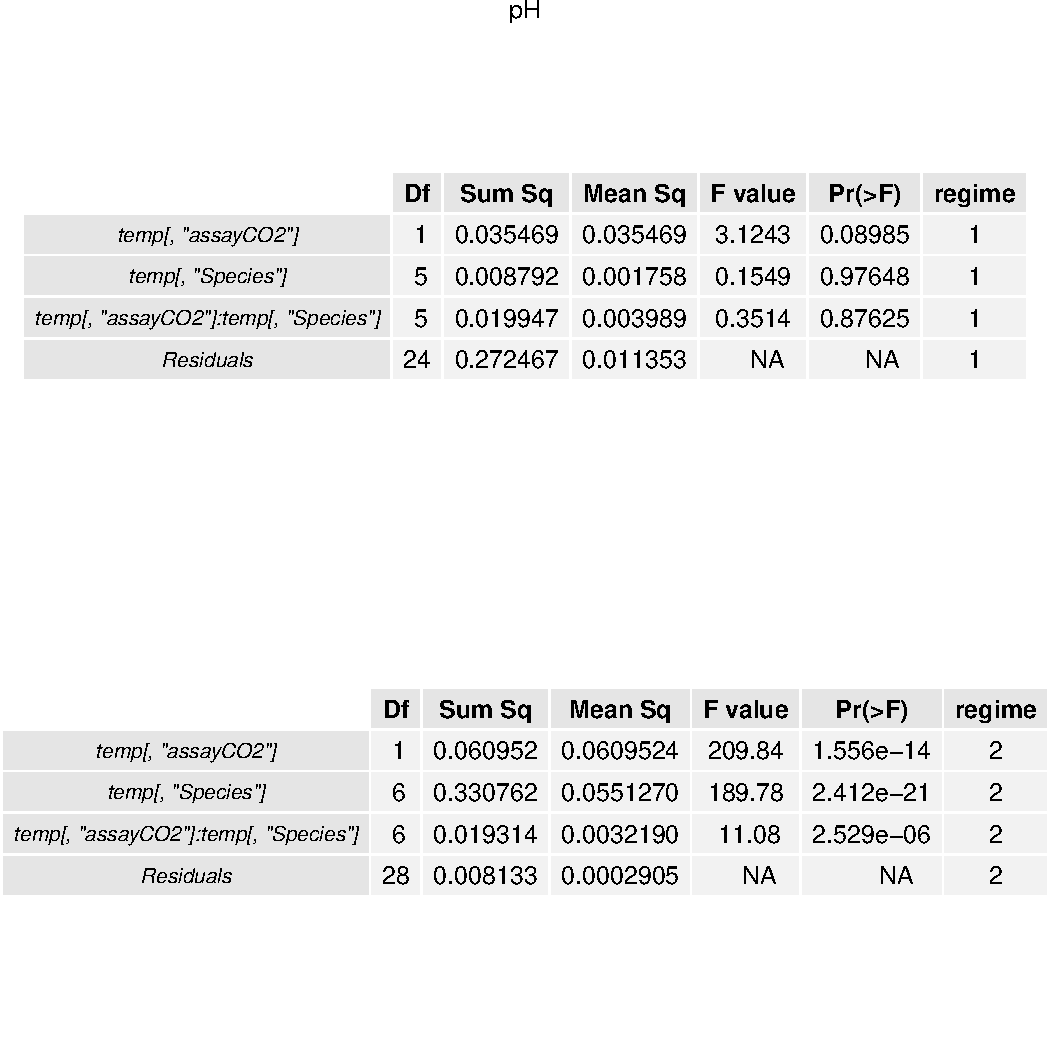
\includegraphics[width=\maxwidth]{figure/physical_parameters_figure11} 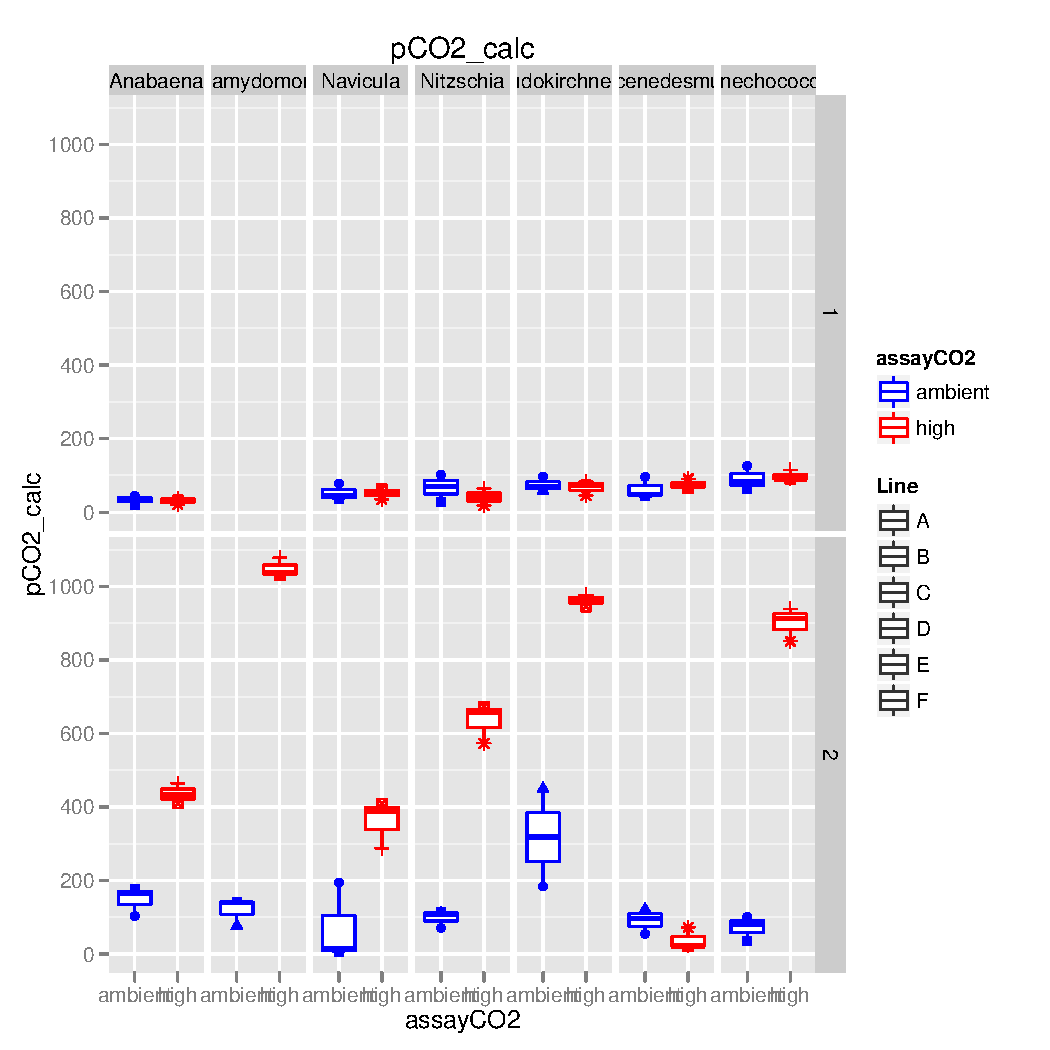
\includegraphics[width=\maxwidth]{figure/physical_parameters_figure12} 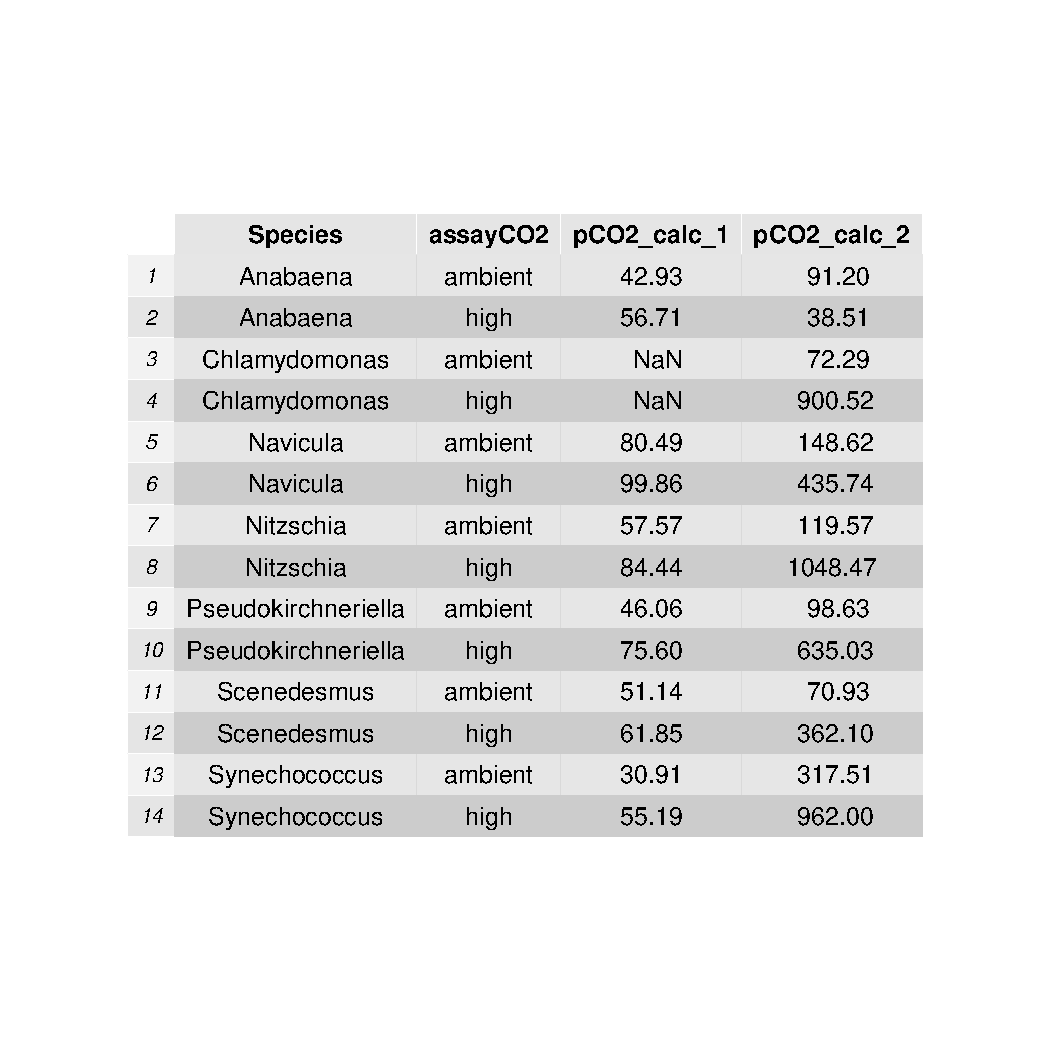
\includegraphics[width=\maxwidth]{figure/physical_parameters_figure13} 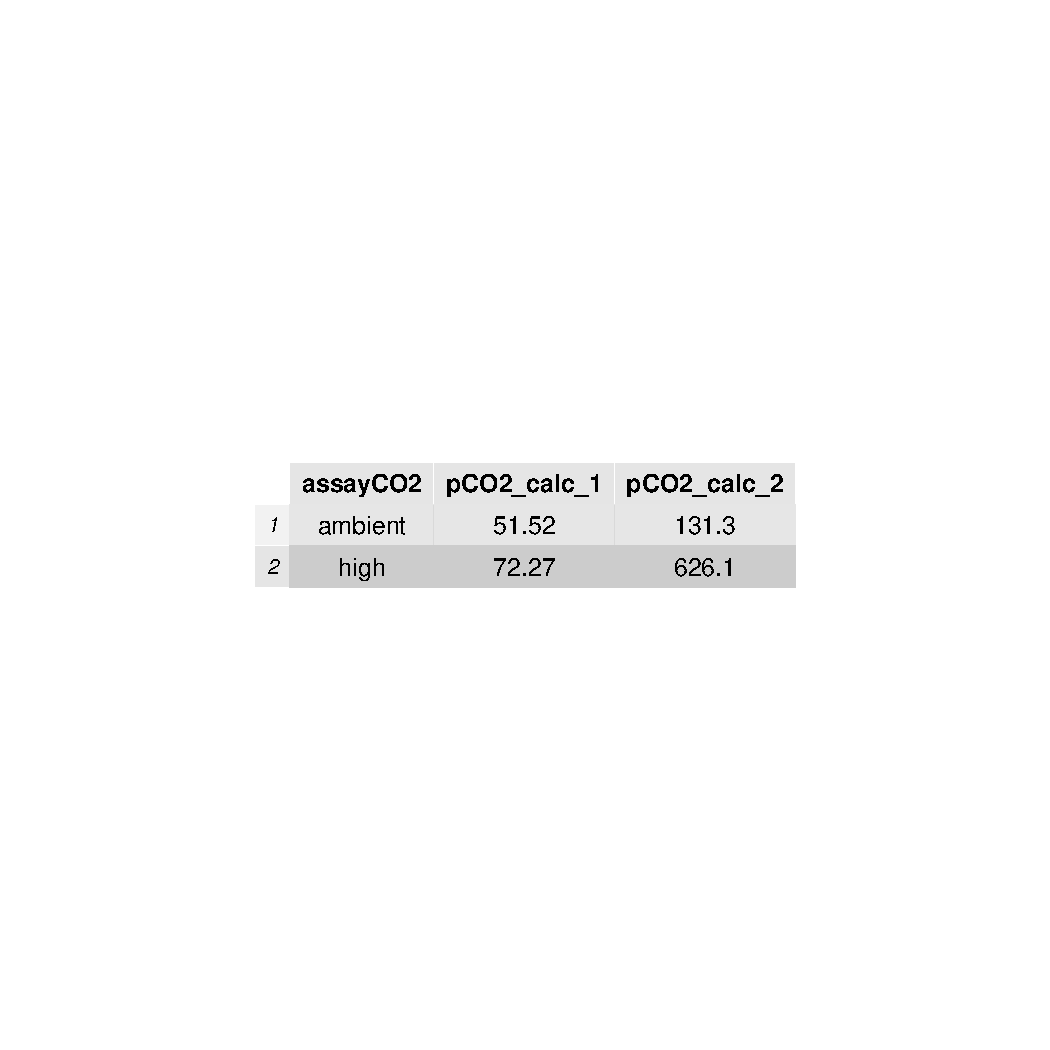
\includegraphics[width=\maxwidth]{figure/physical_parameters_figure14} 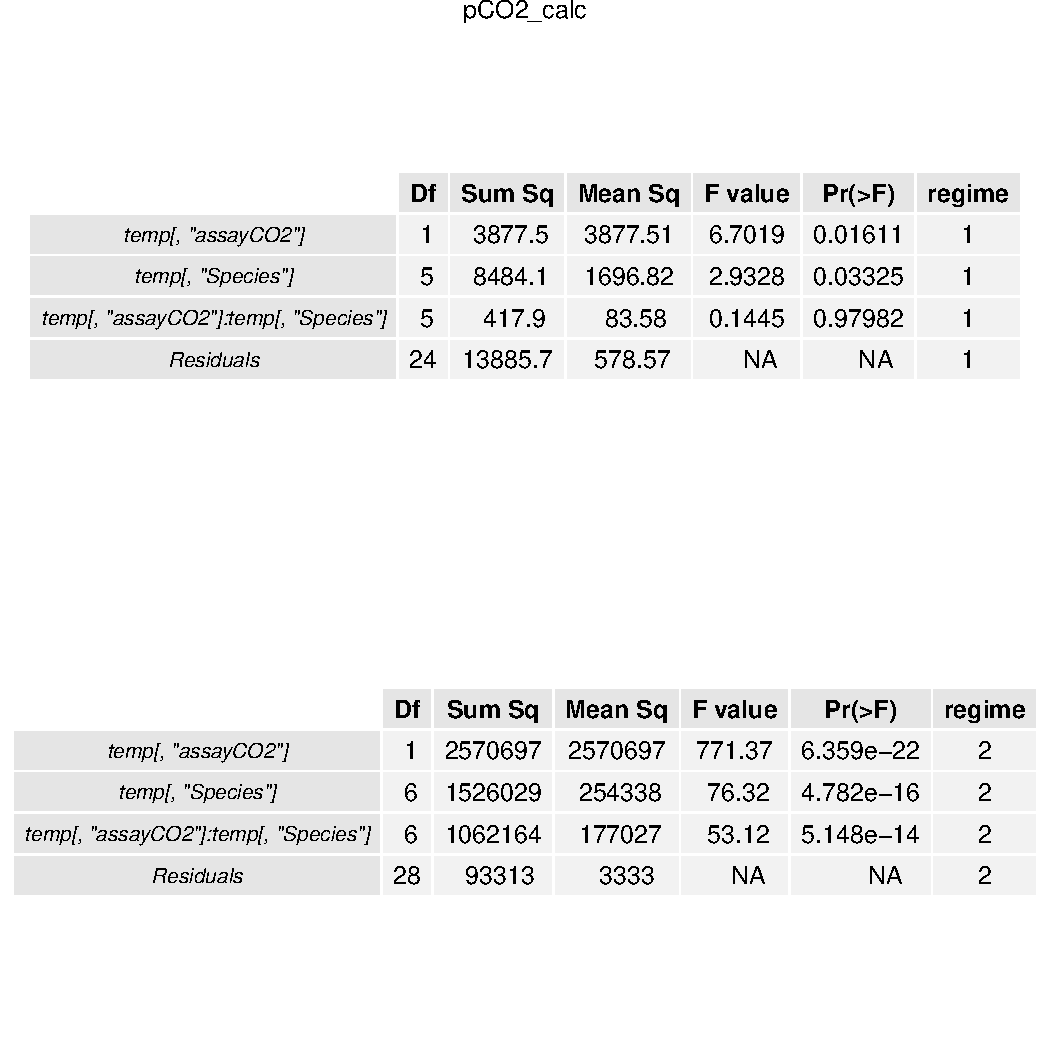
\includegraphics[width=\maxwidth]{figure/physical_parameters_figure15} 
\end{knitrout}




\end{document}
